\documentclass[11pt, a4paper]{article}

\usepackage[utf8]{inputenc}
\usepackage[swedish]{babel}

\usepackage{parskip}
\usepackage{setspace}
\usepackage[babel]{microtype}
\usepackage[labelsep=period, labelfont=bf, textfont=it, skip=5pt]{caption}
\usepackage{dirtytalk}

\usepackage[style=apa, citestyle=apa]{biblatex}
\addbibresource{bibliography.bib}

\usepackage{amsmath}
\usepackage{amsfonts}
\usepackage{siunitx}

\usepackage{svg}
\svgpath{{images/}}
% To include SVG figure:
%\includesvg[inkscapelatex=false, width=\textwidth]{svg_image}

\usepackage{graphicx}
\graphicspath{{images/}}

\title{Magnetisk resonanstomografi}
\author{Björn Sundin\medskip\\\normalsize Fysik 3 - NTI Kronhus}

\begin{document}

\maketitle
\vfill
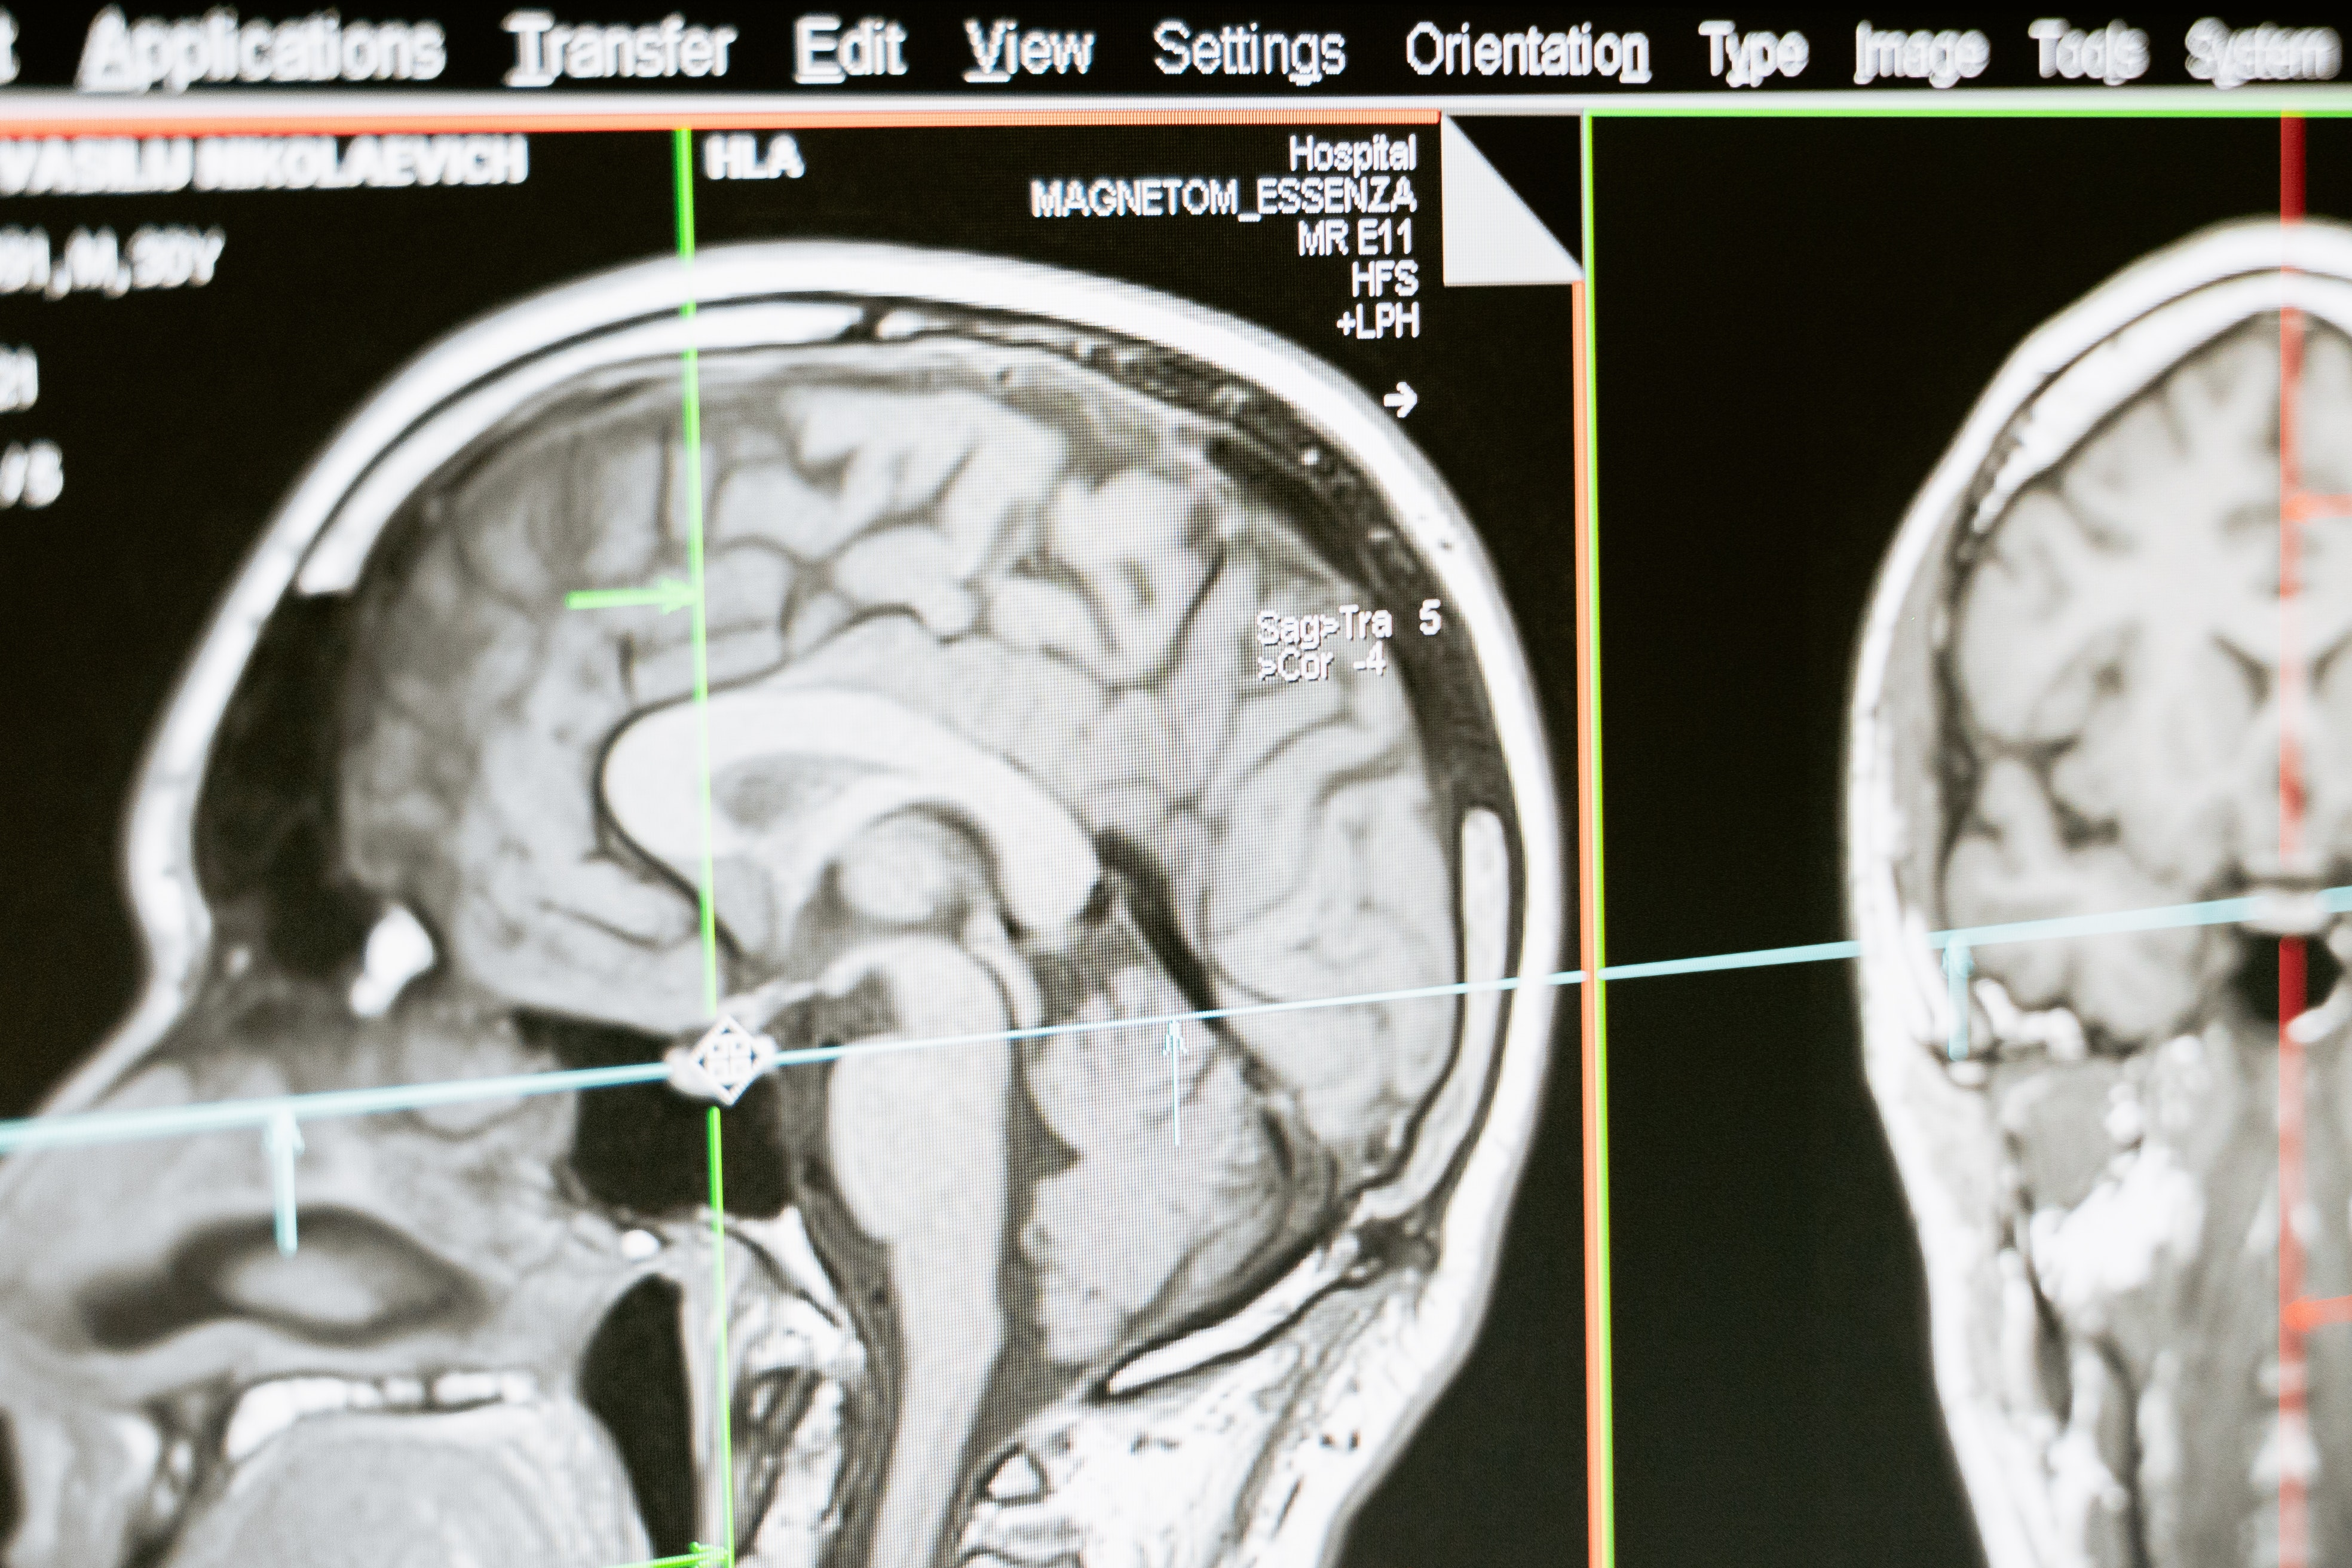
\includegraphics[width=\textwidth]{mri_scan.jpg}
\vspace{1cm}
\vfill

\clearpage
\section{Bakgrund}

Magnetisk resonanstomografi, förkortat MRT eller MRI (Magnetic Resonance Imaging) är en teknik som används inom sjukvården för att ge detaljrika bilder av vävnad och organ hos människor och djur på ett ofarligt och icke-påträngande sätt \parencite{mri_nobelpris_pressmeddelande}. Till skillnad från tidigare tekniker för diagnostisk avbildning såsom röntgen, används ingen joniserande strålning i MRI-undersökningar. Istället används ett mycket starkt magnetfält och radiovåg-pulsar. Tekniken bygger på konceptet av kärnmagnetisk resonans/NMR (Nuclear Magnetic Resonance), vars teori hade sina rötter i upptäckten av protonens spinnegenskaper under 1920-talet \parencite{mri_lärobok}.

Benämningen NMR används främst för det fysikaliska fenomenet och inte längre i sammanhang av diagnostiska undersökningar av individer \parencite{nmr_eller_mri}. \say{Magnetisk resonans} är mindre specifikt än \say{kärnmagnetisk resonans} eftersom det även finns elektronspinnresonans som involverar elektronen och inte atomkärnan. Ordet \say{nuclear} eller prefixet \say{kärn-} förknippas med farliga saker av allmänheten, så man undviker ofta att använda den mer specifika benämningen trots att det bara syftar på att man studerar atomkärnan.

Kärnmagnetisk resonans används även inom kemin för att undersöka strukturen hos olika ämnen \parencite{nmr_kemi}. Då produceras ett NMR-spektra, istället för en 2D- eller 3D-bild, som avslöjar egenskaper hos ämnet. År 1945 utvecklade Felix Bloch och Edward Mills Purcell, med kunskap om kvantmekaniken som utvecklades under 1930-talet och tidigare, de första mätningarna som använde sig av kärnmagnetisk resonans \parencite{mri_lärobok}. De mätte signaler från ett vattenprov och ett paraffinprov, och förklarade dessutom de experimentella och teoretiska detaljerna av NMR. För detta delade Bloch och Purcell nobelpriset i fysik år 1952 \parencite{nmr_nobelpris}.

Två av de främsta utvecklarna av MRI-teknologin var Paul Lauterbur och Peter Mansfield \parencite{mri_nobelpris_pressmeddelande}. Under 1970-talet gjorde Lauterbur och Mansfield flera upptäckter som lade en grund för utvecklingen av MRI. 1973 beskrev Lauterbur hur gradientmagneter kunde användas tillsammans med NMR för att göra flera endimensionella projektioner av ett objekt, som sedan sätts ihop till en två- eller tre-dimensionell bild. I hans experiment kunde han använda tekniken för att skilja på vanligt och tungt vatten, något som ingen annan avbildningsmetod kunde göra. Samma år utnyttjade Mansfield tillsammans med Peter Grannell gradientmagneter med NMR för att undersöka strukturen i fasta ämnen på ett mer exakt sätt. 1977 tog Mansfield fram en ny metod för NMR-avbildning som utnyttjade egenskaperna hos en effekt som kallas spinn-eko i gradientmagneterna. Denna nya metod kunde producera bilder snabbare än tidigare metoder. Lauterbur och Mansfield fick år 2003 nobelpriset i Fysiologi eller Medicin \parencite{mri_nobelpris_pressmeddelande}.

Magnetisk resonanstomografi började tillämpas i sjukvården redan i början av 1980-talet, och år 2002 fanns det mer än 22 000 magnetkameror i hela världen \parencite{mri_nobelpris_pressmeddelande}. Utvecklingen av MRI revolutionerade medicinen, och sedan dess har tekniken fortsatt att utvecklas och förfinas \parencite{mri_facts}. Magnetkameran används för att undersöka alla organ i kroppen

\clearpage
\section{Teori}
%En grundläggande princip som utnyttjas i denna teknik är att energin som detekteras i NMR är proportionell mot magnetfältets styrka. Gradientmagneterna gör att magnetfältets styrka varierar linjärt på en axel, och detta gör alltså att den endimensionella projektionen kan erhållas. 

Kärnan hos väteatomer består av en proton, som har spinnkvanttalet $s=\frac{1}{2}$. Spinnet gör att partikeln beter sig som en magnet med en nordpol och en sydpol. Det magnetiska spinnkvanttalet bestämmer det specifika spinntillståndet och kan ha värdena $m_s=s+n$ där $n\in\{-2s..0\}$. För 

Bara kärnor med ett nollskiljt spinn kan användas för kärnmagnetisk resonans

Spinnkvanttalet $s$ bestämmer ett rörelsemängdsmoment som är speciellt för varje typ av partikel. Endast riktningen av spinnet $m_s$ kan ändras hos en partikel, inte magnituden. Hos en elektron är $s=\frac{1}{2}$ och $m_s=\pm\frac{1}{2}$.

Precession-frekvensen för protonerna bestäms av larmor-ekvationen:
\begin{equation}
    \omega=2\pi f=\gamma B_0\:[\si{rad/s}]
\end{equation}

\clearpage
\section{Användningsområden}


\clearpage
\section{Avslutning}

\clearpage
\printbibliography

\end{document}
